
\documentclass{article}

\usepackage{microtype}
\usepackage{graphicx}
\usepackage{booktabs}
\usepackage{array}
\usepackage{hyperref}
\usepackage{xcolor}
\usepackage[accepted]{icml2025}
\usepackage{amsmath}
\usepackage{enumitem}
\usepackage{tikz}
\usetikzlibrary{positioning,arrows.meta,fit}
\usepackage[capitalize,noabbrev]{cleveref}

\graphicspath{{figures/}}
\makeatletter
\renewcommand{\ICML@appearing}{Course report, Deep Neural Engineering, Open Universiteit, November 2026.}
\makeatother
\newcommand{\todo}[1]{\textcolor{red}{[#1]}}

\icmltitlerunning{GraphRAG versus Vanilla RAG on a Tennis Coaching Corpus}

\begin{document}

\twocolumn[
\icmltitle{GraphRAG versus Vanilla RAG on a Tennis Coaching Corpus\\with Limited Compute}

\begin{icmlauthorlist}
\icmlauthor{Thomas Flamant}{ou}
\end{icmlauthorlist}
\icmlaffiliation{ou}{Open Universiteit, Heerlen, the Netherlands. Student number 852733115}
\icmlcorrespondingauthor{Thomas Flamant}{thomflam@gmail.com}
\icmlkeywords{retrieval-augmented generation, knowledge graphs, GraphRAG, LLM-as-a-judge, tennis coaching}

\vskip 0.3in
]

\printAffiliationsAndNotice{}

\begin{abstract}
Vector retrieval-augmented generation (RAG) struggles with questions that span a whole corpus; GraphRAG
addresses this by building a knowledge graph and community summaries from the text. Edge et al.
evaluated it with gpt-4-turbo on broad corpora, so whether this advantage holds with a smaller, accessible model on limited
compute, in a specialised field, remains open. We compared GraphRAG's local and global search with basic vector RAG on
200 tennis-coaching articles, using Qwen2.5-14B on free Kaggle GPUs and 60 questions of three kinds
(look-up, connecting, big-picture). We evaluated the answers with two LLM judges (Claude Opus 5.5 and Mistral Small 24B),
two human raters and a correctness check against reference notes, and measured the cost. Building on Edge et al., we expected global
search to win on big-picture questions and, further, local search on connecting questions and basic RAG
on look-up questions. Instead, basic RAG beat both GraphRAG systems on almost all criteria and on correctness
(1.77 against 1.37 and 1.13 out of 3), while global search used about 4.6 times the prompt tokens per answer. Our analysis suggests that the
small model and the domain prompt produced a fragmented graph, and that graphrag's default of clustering
only the largest connected component left 66\% of its entities out of the community reports that global
search reads. Under limited compute, basic RAG appears the better choice.
\end{abstract}

\section{Introduction}
\label{sec:intro}

Retrieval-augmented generation (RAG) \cite{lewis2020rag} lets a large language model (LLM) answer
from documents it was not trained on, or from a text collection too large to fit in its context window (the maximum number of tokens it can process at once). 
In its common form, also known as `vector RAG', the system retrieves the text chunks most similar to the query, as many as fit the context window. Vector RAG,
however, struggles with queries that need a global, corpus-wide understanding of the data
(sensemaking), such as the main themes or changing trends across a whole collection
\cite{edge2024local}. GraphRAG \cite{edge2024local} addresses this by building, in advance, a
knowledge graph of the corpus and summaries of its thematic clusters (communities), and also offers
a local search that combines graph elements with the source text.

We use the ITF Coaching \& Sport Science Review, chosen because it is publicly available under an
open CC BY licence. It publishes articles on tennis coaching and sport science, a field the author
knows well.
Unlike the two general-interest corpora of \citet{edge2024local}, podcast
conversations about technology and news articles on many topics, ours covers a single specialised
field. This lets us test whether their method generalises
to narrower domains, a question they leave open.
We deliberately work with limited compute. Building a GraphRAG index with a frontier model through an
API would be costly, so we use a smaller open model, Qwen2.5-14B \cite{qwen2025}, run on free Kaggle
GPUs. This is also a realistic setting: organisations with limited compute and budget, such as a
tennis club or federation, face the same constraint. The constraint weighs more heavily on GraphRAG
than on vector RAG, because GraphRAG needs many more LLM calls to build its knowledge graph and index.
It is therefore an open question whether GraphRAG keeps its advantage when compute is limited.

Building on \citet{edge2024local}, we expect global search to win on big-picture
questions; we further expect local search to perform well on connecting questions, and basic RAG to
do well on look-up questions.
\begin{enumerate}[label=\textbf{H\arabic*},leftmargin=*,nosep]
  \item On big-picture questions, global search beats basic RAG on comprehensiveness and diversity.
  \item On connecting questions, local search beats basic RAG on comprehensiveness and diversity.
  \item Basic RAG beats both local and global search on directness.
  \item On look-up questions, basic RAG beats local and global search on correctness; on connecting
    questions, local search beats basic RAG on correctness.
\end{enumerate}
We also expect GraphRAG to cost more compute than basic RAG, both to index and per answer; we measure
and report this cost but do not test it statistically.

Our contributions are:
\begin{itemize}[leftmargin=*,nosep]
  \item A comparison of GraphRAG and vector RAG on a specialised corpus, coaching and sport-science
    articles, addressing whether the method generalises beyond general-interest data.
  \item An evaluation of GraphRAG's local search, which Edge et al.\ left for future work, alongside
    global search, on three kinds of questions: look-up, connecting and big-picture.
  \item A correctness check against reference notes drafted from the source articles, in addition to the four
    criteria of Edge et al., and checks on the main LLM judge with a second judge from another model
    family and a human sample rated by two people.
  \item A pipeline that runs entirely on a 14B open model on free GPUs, with indexing and per-answer
    cost reported and the code released.
\end{itemize}
\Cref{sec:related} reviews related work, \cref{sec:method} describes the data and method,
\cref{sec:results} reports the results, \cref{sec:discussion} discusses them and
\cref{sec:conclusion} concludes.

\section{Related Work}
\label{sec:related}

Retrieval-augmented generation was introduced by \citet{lewis2020rag} for knowledge-intensive questions
that a model cannot answer from its training alone: before answering, the model retrieves passages from
a large document collection (Wikipedia, in their case) and conditions its answer on them.
Dense passage retrieval (DPR) \cite{karpukhin2020dpr} encodes questions and passages with two neural
encoders into vectors that lie close together when their meanings are similar, even if their words
differ, and retrieves the passages closest to the question; it outperformed keyword retrieval (BM25)
and became the retriever of the original RAG. Our basic system follows this dense-retrieval approach with bge-m3
\cite{chen2024bgem3} as the encoder, filling the context budget with the chunks closest to the
question; local search also starts from vector similarity, but to find entities in the knowledge graph.
\citet{gao2023ragsurvey} distinguish naive, advanced and modular RAG: our basic system is the
naive form, which simply retrieves the most similar chunks, while graph-based methods such as GraphRAG can be seen as
modular RAG, adding a graph to a flexible pipeline of retrieval modules.

GraphRAG \cite{edge2024local} uses an LLM to extract entities, relationships and, optionally, claims
from text chunks, with a ``gleaning'' step that asks the LLM for entities it missed, and merges them
into one knowledge graph. The Leiden algorithm \cite{traag2019leiden} then recursively partitions the
graph into a hierarchy of nested communities: thematic clusters that the LLM summarises in community
reports, from which global search answers.
LightRAG \cite{guo2024lightrag} also builds a graph but has no community reports: it retrieves entities
and relationships directly, combined with vector search, at a specific and a broader level, and is
cheaper to update when new documents arrive. \citet{peng2024graphragsurvey} describe the
whole family in three steps: graph-based indexing, graph-guided retrieval and graph-enhanced
generation.
\citet{han2025ragvsgraphrag} compared vector RAG under one setup with several graph-based
methods, including GraphRAG's local and global search, HippoRAG2 \cite{gutierrez2025hipporag2} and
RAPTOR \cite{sarthi2024raptor}, on question answering and query-based summarisation. Vector RAG was best
on detailed single-hop questions, whose answer sits in one place in the corpus; GraphRAG's local search
did well on multi-hop questions, but its global search often struggled on question answering; and even
for summarisation, methods that retrieve the original text chunks performed well.
Our results agree with theirs: basic RAG was the most correct on our look-up questions, global search
struggled, with the lowest correctness and losses on most criteria, and access to the source text
mattered even for big-picture questions, where basic RAG also performed best. Unlike theirs, however,
our local search lost to basic RAG on connecting, multi-hop questions. Han et al.\ built their graphs with GPT-4o-mini, whose
size is not published but which is likely a stronger extractor than our 4-bit Qwen2.5-14B
(\cref{sec:discussion}). In contrast to both studies, we use a specialised corpus, build the graph with a
small (14B) open model run on free cloud GPUs, and add a correctness check against reference notes.

LLM judges agree with human raters about as often as humans agree with each other
\cite{zheng2023judging}, and so did our raters (\cref{tab:human}). They are, however, biased by the
order in which answers are shown \cite{wang2023fair,han2025ragvsgraphrag} and by answer length
\cite{zheng2023judging,dubois2024length}, and they tend to prefer answers from their own model family
\cite{zheng2023judging}. We therefore judged every pair in both orders, as Wang et al.\ recommend,
measured position consistency and length bias (\cref{sec:discussion}), and avoided self-preference by
generating the answers with Qwen and judging them with Opus and Mistral, models from three different
developers, alongside two human raters.

\citet{strubell2019energy} called for reporting the energy use and cost of NLP models;
following this, we report GPU-hours and kWh for indexing and for answering, and the API cost of judging, whereas
Edge et al.\ report token counts and indexing time, but not energy or GPU-hours.

\section{Data and Method}
\label{sec:method}


\subsection{Corpus and questions}
\label{sec:corpus}
The corpus is the ITF Coaching \& Sport Science Review, the open-access journal of the International
Tennis Federation, published under CC BY. We collected 587 articles (2009--2026) with their metadata.
Text was extracted with PyMuPDF, without running headers and (where the heading was recognised) reference lists, and with a header
(title, authors, year) so that every chunk can be traced to its article. After removing 46 articles
without a PDF or usable text, 541 remain (1.64M tokens). Indexing all of them would take about 34 hours
on our hardware, against Kaggle's limit of 12 hours per session and 30 hours of GPU time per week. The graph is therefore built on a subset of 200 articles (0.59M tokens): the
first 50 usable articles, the 91 source articles of the candidate questions, and a seeded random
sample for the rest.

The evaluation uses 60 questions written from the point of view of a coach who advises adult club
players, 20 of each of three kinds: \emph{look-up} questions, whose answer is in one article;
\emph{connecting} questions, which need several articles; and \emph{big-picture} questions about
themes across the corpus and its years, the kind of global sensemaking question for which GraphRAG
was designed \cite{edge2024local}. An LLM (Claude) drafted a pool of 110 candidate questions from the corpus, each look-up and connecting
question with a short note of the key points a good answer contains, taken from its source article.
The author approved a selection of 60 together with their notes. The questions are
split into a development set of 15 (5 per kind), used for set-up choices such as the
global-search community level,
and a test set of 45 (15 per kind), on which all results are reported.

\subsection{Index and systems}
\label{sec:systems}
\begin{figure}[t]
\centering
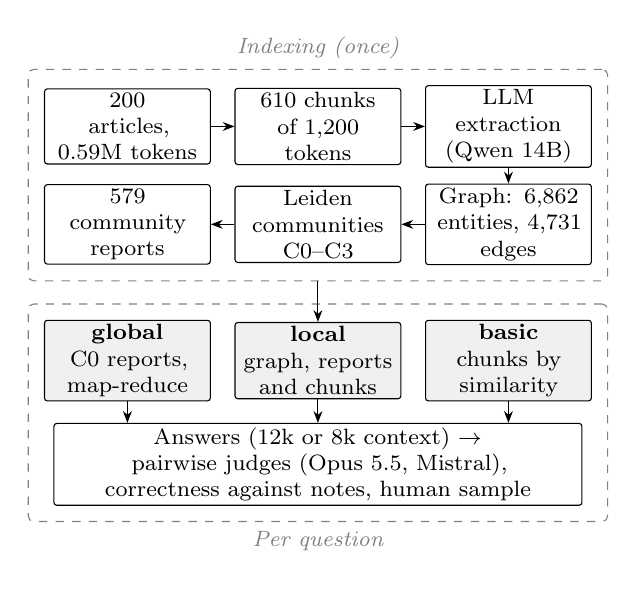
\begin{tikzpicture}[font=\footnotesize, node distance=2mm and 3mm,
  box/.style={draw, rounded corners=1pt, align=center, inner sep=1.5pt, minimum height=6mm, text width=20mm,
    execute at begin node={\hyphenpenalty=10000}},
  sys/.style={box, fill=black!6, minimum height=8mm},
  grp/.style={draw, dashed, gray, rounded corners=2pt, inner sep=2mm},
  arr/.style={-{Stealth[length=1.5mm]}}]
  \node[box] (art) {200\\articles,\\0.59M tokens};
  \node[box, right=of art] (chk) {610 chunks\\of 1,200\\tokens};
  \node[box, right=of chk] (ext) {LLM\\extraction\\(Qwen 14B)};
  \node[box, below=of ext] (gra) {Graph: 6,862\\entities, 4,731\\edges};
  \node[box, left=of gra] (com) {Leiden\\communities\\C0--C3};
  \node[box, left=of com] (rep) {579\\community\\reports};
  \draw[arr] (art) -- (chk); \draw[arr] (chk) -- (ext); \draw[arr] (ext) -- (gra);
  \draw[arr] (gra) -- (com); \draw[arr] (com) -- (rep);
  \node[grp, fit=(art)(ext)(rep)(gra), label={[font=\footnotesize\itshape, gray]above:Indexing (once)}] (idx) {};
  \node[sys, below=7mm of rep] (glo) {\textbf{global}\\C0 reports,\\map-reduce};
  \node[sys, right=of glo] (loc) {\textbf{local}\\graph, reports\\and chunks};
  \node[sys, right=of loc] (bas) {\textbf{basic}\\chunks by\\similarity};
  \node[box, below=3mm of loc, text width=66mm] (eva) {Answers (12k or 8k context) $\rightarrow$\\pairwise judges (Opus 5.5, Mistral),\\correctness against notes, human sample};
  \node[grp, fit=(glo)(bas)(eva), label={[font=\footnotesize\itshape, gray]below:Per question}] (qry) {};
  \draw[arr] (idx.south) -- (loc.north);
  \draw[arr] (glo) -- (glo |- eva.north); \draw[arr] (loc) -- (eva); \draw[arr] (bas) -- (bas |- eva.north);
\end{tikzpicture}
\caption{Pipeline. The index is built once; each question is answered by the three systems (shaded),
which share the chunks, embeddings and answer model.}
\label{fig:pipeline}
\end{figure}
We use Microsoft's \texttt{graphrag} library (version 3.3.0) for indexing, local and global search, and
reimplement its basic search (see Code and Data), so that all three systems share the same chunks, embeddings
and answer model. All generation runs on
Qwen2.5-14B-Instruct with 4-bit AWQ quantisation \cite{qwen2025}, served with vLLM
\cite{kwon2023vllm} on two NVIDIA T4 GPUs (16\,GB each) in Kaggle notebooks; embeddings come from
bge-m3 \cite{chen2024bgem3}. The articles are split into chunks of 1,200 tokens with 100 tokens of
overlap. The LLM extracts entities and relationships with one round of gleaning, and Leiden
communities are summarised in community reports (\cref{fig:pipeline}). Extraction uses a domain prompt with ten entity types (technique, tactic, drill, injury,
physical quality, mental skill, equipment, person, organisation and event) and two hand-written
coaching examples (\cref{sec:prompts}). The resulting graph has 6,862 entities, 4,731 relationships and 579
community reports on four levels, C0 (63 reports) to C3 (\cref{tab:levels}). Following graphrag's
default, only the largest connected component of the graph is clustered into communities, so 2,335 of
the 6,862 entities (34\%) end up in a community; 2,037 entities have no relationship at all.

The three systems answer each question with a single prompt template per system:
\begin{itemize}
\item \textbf{Basic} (the vanilla RAG baseline): the chunks most similar to the question by embedding
similarity, as many as fit the context budget, in one LLM call.
\item \textbf{Local search}: the entities most similar to the question, their relationships, the
community reports they belong to and the chunks that mention them, combined into one context and
answered in one LLM call.
\item \textbf{Global search}: a map-reduce over all community reports of level C0. Each batch of
reports that fits the context budget gives a partial answer with rated key points (map), and the
highest-rated points are combined into the final answer (reduce). Global search reads community
reports only, never the article text.
\end{itemize}
The context budget is 12,000 tokens for all three systems. Because Edge et al. used 8,000 tokens
\cite{edge2024local}, basic and global search were also run with an 8,000-token budget. Global search
uses only level C0: at level C2, a single question took 45 minutes and 412k prompt tokens, against
about 50k tokens at C0. Edge et al.\ found that C0 alone still beat vector RAG on
comprehensiveness and diversity while reading over 97\% fewer tokens than map-reduce over the source
text \cite{edge2024local}; lower levels remain untested here.

The systems are also available as a conversational agent: a follow-up
question is first rewritten by the LLM into a standalone question using the recent conversation, and
then answered by the chosen system, so that the same mechanism serves all three.
\cref{app:dialogue} shows a four-turn dialogue answered by all three systems.

\subsection{Extraction prompt}
\label{sec:prompts}
Before building the main graph, we compared three extraction prompts on the same articles
(\cref{tab:prompts}): graphrag's default prompt with generic entity types (person, organisation, event,
place), the domain prompt described above, and a hybrid of the default prompt with the ten coaching
types. The domain prompt found more entities but fewer relationships than the default prompt, leaving more
entities isolated (41\% against 23\%). Its most connected entities were domain topics such as hygiene
measures and match-fixing, whereas the default prompt's included \emph{coaches}, \emph{ITF} and the
spurious entity ``TABLE~1'', a table caption extracted as an entity. The hybrid prompt left 71\% of its
entities isolated and took three times as long.
We chose the domain prompt for the main graph because its graph centres on domain topics rather than on
generic or noisy entities such as ``TABLE~1'', which better suits coaching questions, at the cost of a
more fragmented graph.

\subsection{Evaluation}
\label{sec:evaluation}
\textbf{Pairwise comparison.} Following \citet{edge2024local}, an LLM judge compares two
answers to the same question on four criteria: \emph{comprehensiveness}, \emph{diversity},
\emph{empowerment} and \emph{directness}, the last serving as a control on which the more focused
vector RAG is expected to win. For each criterion the judge names the better answer or a tie. Every pair of systems is judged on every question in both
display orders, so that position bias \cite{wang2023fair} is balanced. The main judge is Claude Opus 5.5
through the Anthropic API: a frontier model, so that the judgements are not limited by the small
model that generates the answers. A second judge from another model family, Mistral Small 24B Instruct
(AWQ, run locally on the same GPUs), receives the same prompt. Neither judge sees the reference notes.

\textbf{Correctness.} Because the four criteria do not check whether an answer is right, Opus also
grades every answer to the look-up and connecting questions against the reference note of key points:
coverage of all, most, some or none of them (scored 3 to 0), and whether the answer contradicts the
note. Extra material that does not contradict the note is neither rewarded nor penalised. The
big-picture questions have no such note.

\textbf{Human sample.} Twenty answer pairs from the test set (20 different questions, spread over the
three system pairs, with the display order alternated) were rated blind on the same four criteria by
two people independently: the author and a second tennis coach. Citation markers, which would reveal
the system, were replaced by a neutral \texttt{[ref]}.

\textbf{Statistics.} For each question, system pair and criterion, the two verdicts are scored $+1$
(win), $-1$ (loss) or $0$ (tie) and averaged over both display orders. We test whether this score
differs from zero across the 45 test questions with a sign test and with the Wilcoxon signed-rank test
\cite{wilcoxon1945}, which Edge et al. also used, and correct each family of tests (12 per judge at
12k; 8 at 8k, Opus only) with the Holm method \cite{holm1979simple}. A result counts as significant only when both
tests give an adjusted $p < 0.05$. Correctness scores are compared per question with the Wilcoxon
signed-rank test and Holm correction over the three system pairs. Results per question kind (15 test
questions each) are reported descriptively, without significance tests. Agreement between raters is reported
as the share of identical verdicts and as Cohen's $\kappa$ \cite{cohen1960kappa}; for the LLM judges,
the two display orders are netted into one verdict, and a split counts as a tie.
We use the conventional threshold $\alpha = 0.05$. A stricter threshold is not needed to guard
against false positives across the many tests (three system pairs and four criteria per judge),
since the Holm correction already does so.
With 45 test questions, and 15 per kind, the tests can detect only large differences, so a
non-significant result means no evidence of a difference rather than evidence of none.

\textbf{Cost.} We record wall time, GPU-hours (two T4 GPUs over each session's wall time), energy from
the GPUs' reported power draw, and the prompt and generated tokens of every LLM call, both for
indexing and per answer, and the API cost of the Opus judge.

\section{Results}
\label{sec:results}

\begin{table*}[t]
\caption{Pairwise comparison on the test split (45 questions, both display orders), context budget
12k tokens. Each cell is the win rate of the first system of the pair (ties count as half); below 0.5 the
second system wins. * significant after Holm correction with both the sign test and the Wilcoxon
signed-rank test (per question, $\alpha = 0.05$).}
\label{tab:judge12k}
\vskip 0.05in
\begin{center}\begin{small}
\begin{tabular}{llcccc}
\toprule
Judge & Pair (first vs second) & Compr. & Divers. & Empow. & Direct. \\
\midrule
Opus 5.5 & global (12k) vs basic (12k) & 0.24* & 0.40 & 0.11* & 0.22* \\
 & local (12k) vs basic (12k) & 0.24* & 0.36 & 0.26* & 0.26* \\
 & global (12k) vs local (12k) & 0.52 & 0.54 & 0.39 & 0.38 \\
Mistral Small 24B & global (12k) vs basic (12k) & 0.46 & 0.43 & 0.42 & 0.37 \\
 & local (12k) vs basic (12k) & 0.37* & 0.27* & 0.30* & 0.32* \\
 & global (12k) vs local (12k) & 0.55 & 0.57 & 0.63 & 0.49 \\
\bottomrule
\end{tabular}

\end{small}\end{center}
\end{table*}

Across the 45 test questions, the Opus judge preferred basic RAG over both GraphRAG systems on all four
criteria, significantly so on all but diversity (\cref{tab:judge12k}).
H1 is not supported. On the 15 big-picture questions, Opus gave global search a win rate against basic
RAG of 0.23 on comprehensiveness and 0.37 on diversity, and Mistral 0.43 and 0.40, respectively
(\cref{tab:judgebykind}): basic RAG, not global search, was preferred on both criteria. Over all 45
test questions, the corresponding win rates were 0.24 and 0.40 (Opus) and 0.46 and 0.43 (Mistral);
with 45 questions, only the Opus comprehensiveness result was significant.
H2 is not supported either. On the 15 connecting questions, Opus gave local search a win rate against
basic RAG of 0.20 on comprehensiveness and 0.37 on diversity, and Mistral 0.35 and 0.27, respectively:
basic RAG was again preferred on both criteria. Over all 45 test questions, basic RAG's advantage over
local search was significant on comprehensiveness with both judges (0.24 and 0.37) and on diversity
with Mistral (0.27).
H3 is supported: basic RAG beat both GraphRAG systems on directness, with win rates of 0.22 for
global and 0.26 for local search against basic RAG (Opus, both significant). Mistral agreed in
direction (0.37 and 0.32), but only the difference with local search was significant.
Global and local search performed similarly: no difference between them was significant with either
judge (win rates of global over local between 0.38 and 0.63).
With both systems at an 8k-token budget, as in Edge et al., basic RAG was still preferred on
comprehensiveness, empowerment and directness, but only empowerment (0.17) and directness (0.23)
remained significant; on diversity, global search was slightly ahead (0.57, not significant;
\cref{tab:judge8k}).

\begin{table}[t]
\caption{Correctness on the look-up and connecting questions of the test split: coverage of the
reference notes, 0--3 (Opus grader). Contradicts: answers that contradict the notes.}
\label{tab:correctness}
\vskip 0.05in
\begin{center}\begin{small}
\begin{tabular}{lcccc}
\toprule
System & $n$ & Mean (0--3) & SD & Contradicts \\
\midrule
basic (12k) & 30 & 1.77 & 0.86 & 3 \\
local (12k) & 30 & 1.37 & 0.72 & 3 \\
global (12k) & 30 & 1.13 & 0.57 & 7 \\
basic (8k) & 30 & 1.67 & 0.88 & 3 \\
global (8k) & 30 & 1.13 & 0.63 & 5 \\
\bottomrule
\end{tabular}

\end{small}\end{center}
\end{table}

H4 is half supported. On look-up questions, basic RAG was the most correct system, with a mean
score of 1.93 out of 3 against 1.33 for local and 1.00 for global search
(\cref{tab:correctnessbykind}). On connecting questions, however, local search (1.40) did not beat
basic RAG (1.60). Over all 30 questions with reference notes, basic RAG was significantly more correct
than local ($p = 0.010$) and global search ($p = 0.005$), while local and global search did not differ
significantly ($p = 0.090$; \cref{tab:correctness,tab:correctnesstests}). The difference between
basic and global search remained significant at 8k ($p = 0.014$). Global search also contradicted the
reference notes most often (7 of 30 answers, against 3 each for basic and local).

The two human raters agreed only fairly, on the scale of \citet{landis1977measurement} (agreement 0.51,
$\kappa = 0.23$; \cref{tab:human}). This is about as well as each agreed with the LLM judges ($\kappa$
between 0.12 and 0.28), and as the two LLM judges agreed with each other on this sample ($\kappa = 0.30$).
On the full test split, the two LLM judges agreed about as well (agreement 0.52, $\kappa = 0.28$;
\cref{tab:judgeagreement}). All four
raters gave basic RAG the most wins (\cref{tab:humanwins}), in line with the pairwise results. With
20 answer pairs, the sample is a check on the LLM judges rather than a test of the hypotheses.

As expected, GraphRAG cost more. Its index took 24.3 GPU-hours on 2$\times$T4 for 200 articles
(1.56 kWh; \cref{tab:compute}), most of it for LLM extraction, whereas basic RAG needs only the chunk
embeddings. Per answer, global search used about 4.6 times the prompt tokens of basic RAG (49.8k against
10.8k), five LLM calls instead of one, and more time (520 against 294 seconds), while local
search used slightly fewer tokens than basic RAG (9.4k; \cref{tab:costanswer}). Indexing cost grew
roughly in proportion to corpus size, at 3.9--6.3 GPU-hours per 100k tokens (\cref{tab:graphsize}).

\section{Discussion}
\label{sec:discussion}

Unlike \citet{edge2024local}, we found that basic RAG beat both GraphRAG systems. One
likely reason is the model: Qwen2.5-14B, compressed to 4 bits, is less capable than the gpt-4-turbo used
by Edge et al., for which GraphRAG's prompts were written. In our 50-article pilot, 41\% of the
extracted entities had no relationship, some had the wrong type (match-fixing as an injury), and
inconsistent naming (underscores against spaces) kept duplicates from being merged; the final graph has
on average 1.35 connections per entity. This matters most for local search, which finds the entities
closest to the question and then follows their relationships: a connecting question needs links
between articles, and where those links are missing, local search falls back on the few source chunks
it also includes. We do not know how connected the graphs of Edge et al.\ were, however; only a
re-index with a larger model could show whether the model was the main cause. Our domain prompt also played a part: on the same pilot articles, the default prompt left 23\% of the
entities isolated, against 41\% (\cref{sec:prompts}).

A second reason is that global search never sees the source text: it answers from community reports,
which summarise entity descriptions, which in turn summarise what was extracted from the chunks.
Following one concept through the pipeline shows what this can lose. The split step is discussed in 8
chunks from 6 articles. Qwen extracted it as three separate entities (plus three
take-off variants), \textsc{split-step},
\textsc{split step} and \textsc{reactive decision step (split-step)}, which were never merged because
their names differ. Only one of the 63 C0 reports mentions the split step, in a single paragraph based
on one of these entities, so a global answer about it would rest on that short summary, while basic RAG
retrieves the source chunks themselves. The loss is larger than this example suggests: by default,
graphrag clusters only the largest connected part of the graph into communities, so 2,335 of the
6,862 entities (34\%) appear in a community report, and the rest are invisible to global search. This
could explain why global search had the lowest correctness and the most contradictions, and lost on
comprehensiveness, which rewards detail. Missing source text is not the whole story, however: local
search saw source chunks and still lost to basic RAG.

Basic RAG beat GraphRAG in nearly every comparison, across raters and measures. Over the 45 test
questions, the differences are significant at the $\alpha = 0.05$ level justified in \cref{sec:evaluation}:
Opus preferred basic RAG over both GraphRAG systems on comprehensiveness, empowerment and directness,
Mistral preferred it over local search on all four criteria, and basic RAG was more correct than local
and global search ($p = 0.010$ and $0.005$). Diversity with Opus, global search against basic RAG with
Mistral, and all results per question kind (15 questions each, descriptive only) are not significant.
The overall picture is nevertheless consistent, because several measures point the same way: two LLM
judges from different model families, two human raters, and the correctness check against the reference
notes. These measures are not fully independent, however: Opus also grades correctness, Claude, the main judge's family, drafted the questions and notes from specific articles, which may favour basic RAG, the LLM judges saw the
citation markers that reveal each system (the human raters did not), one human rater is the author, and the second rater's wins were nearly even (basic 25, local 22; \cref{tab:humanwins}). Agreement among the raters was
low to fair ($\kappa$ between 0.12 and 0.30 on the human sample), so single verdicts are noisy.
Judging both display orders balances position bias, which was substantial for Mistral: it gave the same
verdict in both orders in 50\% of comparisons, against 80\% for Opus (all 60 questions). On
comprehensiveness, diversity and empowerment the longer answer won 58--73\% of decided verdicts
(\cref{tab:lengthbias}), but the systems' answers were similar in length (586 to 638 tokens on
average), so length bias is unlikely to explain basic RAG's lead. Each pair was judged once
per display order, whereas Edge et al.\ judged each five times; our USD 20 API budget
did not allow more.

Four changes could give GraphRAG a fairer test. The first three reuse the existing extraction, which was
the expensive step. First, clustering the whole graph rather than its largest connected component would
make most of the 36\% of entities in smaller connected components visible to global search; the 30\%
without any relationship would remain isolated. Second, duplicate entities could be merged before the
communities are formed, for example by normalising their names or comparing their descriptions. Third,
big-picture questions could be answered from the 329 smaller C1 reports instead of the 63 at C0, at
about four times the report tokens (\cref{tab:levels}). The fourth, re-indexing with a larger extraction model, is the only direct test of whether the model was
the main cause, but needs more GPU memory than two T4s, or API credits.


\section{Conclusion}
\label{sec:conclusion}

We compared GraphRAG's local and global search with vector RAG on 200 tennis-coaching articles, using
a 14B open model (Qwen2.5) on free Kaggle T4 GPUs. Contrary to Edge et al., basic RAG beat both
GraphRAG systems on almost all criteria and on correctness, at lower cost: H1, H2 and the connecting
half of H4 were not supported, while H3 was. Our analysis suggests that a likely cause is a fragmented graph (small model,
domain prompt) that, with graphrag's largest-component default, left 66\% of the entities out of the
community reports that global search reads.
Beyond the fixes in \cref{sec:discussion}, four directions follow from this study. First, LightRAG
\cite{guo2024lightrag} retrieves graph entities and relationships directly instead of community reports,
skipping the step where most of our entities were lost, at a lower indexing cost. Second, a hybrid
system could give the answer model both the source chunks that carried basic RAG's detail and the graph
connections that connecting questions need. Third, a larger evaluation, with more big-picture questions,
more human raters and repeated judging, could detect smaller differences than our 15 questions per kind.
Finally, the conversational agent could be built on the best system and tested with coaches on their own
questions, the setting of limited budgets that motivated this study.

\section*{Code and Data}
\label{sec:code}
The code is available at \url{https://github.com/tom8to888/dne-graphrag}. New relative to the \texttt{graphrag} library are:
a Kaggle pipeline that runs indexing, querying, the conversational agent and the
second judge; a fix for the empty answers of graphrag~3.3's basic search; the pairwise judge, the
correctness grader and the statistics; and the code that draws the blinded human sample. A README and
\texttt{run\_all.sh} reproduce every stage and table.

\bibliography{references}
\bibliographystyle{icml2025}

\section*{Use of AI}
AI (Claude, Anthropic) was used as a coding and writing assistant.
Separately, LLMs are objects of study here: Qwen2.5-14B generates the answers, and Claude Opus 5.5
and Mistral Small 24B act as judges.

\newpage
\appendix
\onecolumn

\section{Additional Results}
\label{app:results}

\begin{table}[h]
\caption{Human sample: 20 blinded answer pairs from the test split, four criteria each (80 verdicts
per pair of raters). Agreement on the verdict (first, second or tie) and Cohen's $\kappa$. The LLM
judges' verdicts net both display orders.}
\label{tab:human}
\vskip 0.05in
\begin{center}\begin{small}
\begin{tabular}{lccc}
\toprule
Raters & Verdicts & Agreement & $\kappa$ \\
\midrule
Human 1 vs Human 2 & 80 & 0.51 & 0.23 \\
Human 1 vs Opus & 80 & 0.55 & 0.28 \\
Human 1 vs Mistral & 80 & 0.51 & 0.28 \\
Human 2 vs Opus & 80 & 0.45 & 0.12 \\
Human 2 vs Mistral & 80 & 0.47 & 0.21 \\
Opus vs Mistral & 80 & 0.53 & 0.30 \\
\bottomrule
\end{tabular}

\end{small}\end{center}
\end{table}

\begin{table*}[t]
\caption{Cost per answer (mean over the 60 questions). Prompt tokens include the retrieved context, as counted
by graphrag; vLLM's totals, which add the question and the chat template, are about 7\% higher;
latency is wall time per answer with three questions answered at once on 2$\times$T4. Articles: distinct
source articles in the context.}
\label{tab:costanswer}
\vskip 0.05in
\begin{center}\begin{small}
\begin{tabular}{lccccc}
\toprule
System & LLM calls & Prompt tok. & Answer tok. & Latency (s) & Articles \\
\midrule
basic (12k) & 1 & 10,767 & 638 & 294 & 6.9 \\
local (12k) & 1 & 9,405 & 605 & 340 & 4.2 \\
global (12k) & 5 & 49,817 & 586 & 520 & 0.0 \\
basic (8k) & 1 & 8,047 & 607 & 228 & 5.2 \\
global (8k) & 7 & 51,895 & 616 & 368 & 0.0 \\
\bottomrule
\end{tabular}

\end{small}\end{center}
\end{table*}

\begin{table}[h]
\caption{Pairwise comparison at an equal 8k-token context budget (Opus judge, test split), and global
search at 8k against 12k. Cells and * as in \cref{tab:judge12k}.}
\label{tab:judge8k}
\vskip 0.05in
\begin{center}\begin{small}
\begin{tabular}{lcccc}
\toprule
Pair (first vs second) & Compr. & Divers. & Empow. & Direct. \\
\midrule
global (8k) vs basic (8k) & 0.39 & 0.57 & 0.17* & 0.23* \\
global (8k) vs global (12k) & 0.62 & 0.64 & 0.57 & 0.47 \\
\bottomrule
\end{tabular}

\end{small}\end{center}
\end{table}

\begin{table}[h]
\caption{Paired comparison of correctness per question (Wilcoxon signed-rank, Holm-corrected within
each run). Better/Worse: questions where the first system scored higher/lower.}
\label{tab:correctnesstests}
\vskip 0.05in
\begin{center}\begin{small}
\begin{tabular}{lccccc}
\toprule
Pair & Better & Worse & Equal & Mean diff. & $p_\text{Holm}$ \\
\midrule
basic (12k) vs local (12k) & 11 & 1 & 18 & +0.40 & 0.010 \\
basic (12k) vs global (12k) & 15 & 2 & 13 & +0.63 & 0.005 \\
local (12k) vs global (12k) & 10 & 4 & 16 & +0.23 & 0.090 \\
basic (8k) vs global (8k) & 14 & 3 & 13 & +0.53 & 0.014 \\
basic (8k) vs basic (12k) & 6 & 8 & 16 & $-$0.10 & 0.934 \\
global (8k) vs global (12k) & 3 & 3 & 24 & +0.00 & 1.000 \\
\bottomrule
\end{tabular}

\end{small}\end{center}
\end{table}

\begin{table}[h]
\caption{Human sample: verdicts won per system (decided verdicts) and share of ties, per rater.}
\label{tab:humanwins}
\vskip 0.05in
\begin{center}\begin{small}
\begin{tabular}{lcccc}
\toprule
Rater & basic & local & global & Ties \\
\midrule
Human 1 & 37 & 12 & 13 & 22\% \\
Human 2 & 25 & 22 & 13 & 25\% \\
Opus & 42 & 18 & 9 & 14\% \\
Mistral & 26 & 7 & 15 & 40\% \\
\bottomrule
\end{tabular}

\end{small}\end{center}
\end{table}

\begin{table}[h]
\caption{Compute per stage. GPU-hours count both T4 GPUs over the session's wall time, including about
10--16 minutes of set-up per session; energy from the GPUs' reported power draw. The 12k answers exclude
a 1.1 GPU-hour benchmark session that produced 12 of the 180 answers.}
\label{tab:compute}
\vskip 0.05in
\begin{center}\begin{small}
\begin{tabular}{lccc}
\toprule
Stage & GPU-h (T4) & kWh & API (USD) \\
\midrule
Indexing, 200 articles (2 sessions) & 24.3 & 1.56 & -- \\
Answers, 3 systems $\times$ 60 q. (12k) & 13.4 & 0.82 & -- \\
Answers, 2 systems $\times$ 60 q. (8k) & 6.96 & 0.45 & -- \\
Second judge (Mistral, local) & 0.93 & 0.05 & -- \\
Opus judge + correctness & -- & -- & 15.68 \\
\bottomrule
\end{tabular}

\end{small}\end{center}
\end{table}

\begin{table}[h]
\caption{Community levels of the 200-article graph. Global search in this report uses C0.}
\label{tab:levels}
\vskip 0.05in
\begin{center}\begin{small}
\begin{tabular}{lccc}
\toprule
Level & Reports & Report tokens & Tokens vs C0 \\
\midrule
C0 & 63 & 42,709 & 1.0 \\
C1 & 329 & 177,681 & 4.2 \\
C2 & 184 & 88,554 & 2.1 \\
C3 & 3 & 1,275 & 0.0 \\
\bottomrule
\end{tabular}

\end{small}\end{center}
\end{table}

\begin{table*}[t]
\caption{Pairwise comparison per question kind (test split, 15 questions per kind, both display orders,
12k context). Each cell is the win rate of the first system of the pair (ties count as half); below 0.5 the
second system wins. Descriptive only: no significance tests per kind.}
\label{tab:judgebykind}
\vskip 0.05in
\begin{center}\begin{small}
\begin{tabular}{lllcccc}
\toprule
Judge & Kind & Pair (first vs second) & Compr. & Divers. & Empow. & Direct. \\
\midrule
Opus 5.5 & big-picture & global vs basic & 0.23 & 0.37 & 0.13 & 0.10 \\
 &  & global vs local & 0.50 & 0.45 & 0.50 & 0.50 \\
 &  & local vs basic & 0.33 & 0.43 & 0.27 & 0.17 \\
 & connecting & global vs basic & 0.27 & 0.40 & 0.10 & 0.23 \\
 &  & global vs local & 0.57 & 0.53 & 0.40 & 0.43 \\
 &  & local vs basic & 0.20 & 0.37 & 0.27 & 0.20 \\
 & look-up & global vs basic & 0.23 & 0.43 & 0.10 & 0.33 \\
 &  & global vs local & 0.50 & 0.63 & 0.27 & 0.20 \\
 &  & local vs basic & 0.20 & 0.27 & 0.23 & 0.40 \\
Mistral Small 24B & big-picture & global vs basic & 0.43 & 0.40 & 0.43 & 0.37 \\
 &  & global vs local & 0.48 & 0.53 & 0.60 & 0.55 \\
 &  & local vs basic & 0.42 & 0.33 & 0.37 & 0.22 \\
 & connecting & global vs basic & 0.48 & 0.37 & 0.42 & 0.43 \\
 &  & global vs local & 0.52 & 0.50 & 0.63 & 0.48 \\
 &  & local vs basic & 0.35 & 0.27 & 0.30 & 0.40 \\
 & look-up & global vs basic & 0.47 & 0.53 & 0.40 & 0.30 \\
 &  & global vs local & 0.65 & 0.67 & 0.67 & 0.43 \\
 &  & local vs basic & 0.35 & 0.22 & 0.23 & 0.33 \\
\bottomrule
\end{tabular}

\end{small}\end{center}
\end{table*}

\begin{table}[h]
\caption{Correctness per question kind: mean score against the reference notes, 0--3 (Opus grader,
test split, 12k). Contradicts: answers that contradict the notes. Big-picture questions have no
reference notes. Descriptive only.}
\label{tab:correctnessbykind}
\vskip 0.05in
\begin{center}\begin{small}
\begin{tabular}{lccccc}
\toprule
Kind & $n$ & basic & local & global & Contradicts (b/l/g) \\
\midrule
connecting & 15 & 1.60 & 1.40 & 1.27 & 1/0/2 \\
look-up & 15 & 1.93 & 1.33 & 1.00 & 2/3/5 \\
\bottomrule
\end{tabular}

\end{small}\end{center}
\end{table}

\begin{table}[h]
\caption{Extraction prompts compared on the same articles (pilot runs). In brackets: number of
articles. $^a$Cut from the 50-article graph. $^b$Inflated by a missing output limit: a few
extraction calls looped until the context was full and were retried (fixed before all later runs).}
\label{tab:prompts}
\vskip 0.05in
\begin{center}\begin{small}
\begin{tabular}{lccccc}
\toprule
 & domain (50) & default (50) & domain (10)$^a$ & default (10) & hybrid (10) \\
\midrule
Entities & 1,608 & 1,276 & 274 & 224 & 877 \\
Relationships & 847 & 1,218 & 203 & 247 & 279 \\
Relationships per entity & 0.53 & 0.95 & 0.74 & 1.10 & 0.32 \\
Isolated entities & 41\% & 23\% & 21\% & 20\% & 71\% \\
Community reports & 38 & 151 & -- & 10 & 34 \\
Extraction time (s) & 12,734$^b$ & 7,096 & -- & 901 & 2,929 \\
\bottomrule
\end{tabular}

\end{small}\end{center}
\end{table}

\begin{table*}[t]
\caption{Indexing cost against corpus and graph size (2$\times$T4, Qwen2.5-14B; the smaller corpora are
the first 10 and 50 articles of the 200). GPU-h = 2 GPUs $\times$ wall time, including start-up.
$^a$Inflated by the missing output limit (\cref{tab:prompts}). $^b$Includes a repeated
community-report stage after a stopped session.}
\label{tab:graphsize}
\vskip 0.05in
\begin{center}\begin{small}
\begin{tabular}{rrlrrrrrr}
\toprule
Articles & Tokens & Prompt & Entities & Relations & Reports & GPU-h & kWh & GPU-h / 100k tok. \\
\midrule
10 & 25,789 & default & 224 & 247 & 10 & 1.0 & 0.05 & 3.9 \\
50 & 121,895 & default$^b$ & 1,276 & 1,218 & 151 & 6.9 & 0.43 & 5.6 \\
50 & 121,895 & domain$^a$ & 1,608 & 847 & 38 & 7.7 & 0.50 & 6.3 \\
200 & 589,594 & domain & 6,862 & 4,731 & 579 & 24.3 & 1.56 & 4.1 \\
\bottomrule
\end{tabular}

\end{small}\end{center}
\end{table*}

\begin{table}[h]
\caption{Length bias: share of decided verdicts won by the longer answer, per criterion and judge (all 60
questions, development and test).}
\label{tab:lengthbias}
\vskip 0.05in
\begin{center}\begin{small}
\begin{tabular}{lccc}
\toprule
Criterion & Opus (12k) & Mistral (12k) & Opus (8k) \\
\midrule
comprehensiveness & 0.66 & 0.64 & 0.72 \\
diversity & 0.66 & 0.73 & 0.66 \\
empowerment & 0.61 & 0.68 & 0.58 \\
directness & 0.45 & 0.45 & 0.40 \\
\bottomrule
\end{tabular}

\end{small}\end{center}
\end{table}

\begin{table}[h]
\caption{Agreement between the two LLM judges (Opus and Mistral), test split, three pairs at 12k; both display orders netted into one verdict per question, pair and criterion.}
\label{tab:judgeagreement}
\vskip 0.05in
\begin{center}\begin{small}
\begin{tabular}{lccc}
\toprule
Criterion & Verdicts & Agreement & $\kappa$ \\
\midrule
comprehensiveness & 270 & 0.48 & 0.24 \\
directness & 270 & 0.60 & 0.42 \\
diversity & 270 & 0.73 & 0.59 \\
empowerment & 270 & 0.61 & 0.39 \\
all & 1080 & 0.61 & 0.41 \\
\bottomrule
\end{tabular}

\end{small}\end{center}
\end{table}

\clearpage
\makeatletter\setlength{\@fptop}{0pt}\makeatother
\section{Demo Dialogue}
\label{app:dialogue}
One of four demo dialogues, run through the conversational agent with each system on the same index
(Qwen2.5-14B, 12k context). Each system rewrites the follow-up questions itself, so the rewritten
questions differ slightly. \Cref{tab:dialoguereading} gives a qualitative reading of the answers and
\cref{tab:dialogue,tab:dialogue2} a verbatim excerpt of each; the full answers of all four dialogues are in
\texttt{results/chat\_demo.md}.

\begin{table}[!ht]
\caption{Qualitative reading of the demo-dialogue answers (\cref{tab:dialogue}; not scored, not part of the
evaluation). Bold: the strongest answer to that turn; turn 1 has no clear best.}
\label{tab:dialoguereading}
\vskip 0.05in
\begin{center}\begin{footnotesize}
\begin{tabular}{p{0.05\textwidth}p{0.28\textwidth}p{0.28\textwidth}p{0.28\textwidth}}
\toprule
Turn & Basic & Local & Global \\
\midrule
1 & Quotes its sources, but the quotes often do not support the claim next to them
  & Concise and on topic, but generic (self-talk, visualisation); adds showing respect to the opponent
  & On topic: a neutral stance and emotional detachment; one off-topic item (perceptual drills) \\[2pt]
2 & Gives strategies but no yes or no
  & Clear yes; weak support (positive environments for young athletes)
  & \textbf{Clear yes, explained by emotional contagion and loss of concentration} \\[2pt]
3 & \textbf{States that the data has no explicit guidance, then gives a balanced view, though it stretches its sources}
  & Balanced: light conversation, but no emotionally charged topics
  & Now recommends conversation, citing 11 reports; sits uneasily with its turn-2 answer \\[2pt]
4 & \textbf{Most targeted ideas: rehearse the opponent's tactics in simulated matches, learn from champions' interviews; all from one source}
  & One practical point, not showing frustration, which would satisfy the opponent; otherwise general mental skills
  & Generic; includes interval training as a defence against mind games \\
\bottomrule
\end{tabular}
\end{footnotesize}\end{center}
\end{table}

\begin{table}[!ht]
\caption{Demo dialogue, turns 1 and 2: the user's turns, each system's rewritten question and an excerpt of
its answer, quoted verbatim. Turn 1 is not rewritten. Words: length of the full answer.}
\label{tab:dialogue}
\vskip 0.05in
\begin{center}\begin{footnotesize}
{\renewcommand{\arraystretch}{1.1}
\begin{tabular}{@{}>{\raggedright\arraybackslash}p{0.07\textwidth}>{\raggedright\arraybackslash}p{0.30\textwidth}>{\raggedright\arraybackslash}p{0.49\textwidth}r@{}}
\toprule
System & Question as rewritten by the system & Answer: section headings (turns 1, 4) or the sentences that answer (turns 2, 3) & Words \\
\midrule
\multicolumn{4}{@{}>{\raggedright\arraybackslash}p{0.97\textwidth}@{}}{\textbf{Turn 1.} \textbf{User:} A club player struggles when his opponent gets emotional, overly tense or displays a negative attitude during match play. What mental strategies exist to handle this?} \\
\addlinespace[3pt]
\textsc{basic} & -- & Maintain Your Focus \,$\cdot$\, Utilize Deep Breathing Techniques \,$\cdot$\, Adapt Your Strategy Based on the Situation \,$\cdot$\, Stay Committed to Your Goals \,$\cdot$\, Use Positive Self-Talk \,$\cdot$\, Leverage Turning Points Strategically & 532 \\
\addlinespace[4pt]
\textsc{local} & -- & Maintain Composure \,$\cdot$\, Focus on Your Game Plan \,$\cdot$\, Use Positive Self-Talk \,$\cdot$\, Visualize Success \,$\cdot$\, Manage Emotions \,$\cdot$\, Show Respect & 330 \\
\addlinespace[4pt]
\textsc{global} & -- & Maintaining Present-Moment Awareness \,$\cdot$\, Neutral Stance and Emotional Detachment \,$\cdot$\, Developing Mental Resilience \,$\cdot$\, Confidence Building and Positive Mindset \,$\cdot$\, Emotional Regulation Techniques \,$\cdot$\, Specific Drills and Perceptual Skills \,$\cdot$\, Stress Management Strategies & 504 \\
\midrule
\multicolumn{4}{@{}>{\raggedright\arraybackslash}p{0.97\textwidth}@{}}{\textbf{Turn 2.} \textbf{User:} Should the player avoid interaction with the opponent during changeovers?} \\
\addlinespace[3pt]
\textsc{basic} & \emph{Should a club player avoid interacting with an opponent who is emotionally turbulent, overly tense, or displaying a negative attitude during changeovers?} & ``When dealing with an opponent who displays these emotional states, it is beneficial for club players to employ specific interaction strategies during changeovers.'' & 460 \\
\addlinespace[4pt]
\textsc{local} & \emph{Is it advisable for the player to avoid interacting with an emotionally charged opponent during changeovers?} & ``Therefore, it is advisable for players to avoid engaging with emotionally charged opponents during changeovers to preserve their mental and emotional stability, which can directly impact their performance.'' & 194 \\
\addlinespace[4pt]
\textsc{global} & \emph{Is it advisable for the player to avoid interacting with an emotionally charged opponent during changeovers in order to maintain focus and performance?} & ``Avoiding interaction with an emotionally charged opponent during changeovers is advisable for maintaining focus and performance.'' & 309 \\
\bottomrule
\end{tabular}}

\end{footnotesize}\end{center}
\end{table}

\begin{table}[!t]
\caption{Demo dialogue, continued: turns 3 and 4 (columns as in \cref{tab:dialogue}).}
\label{tab:dialogue2}
\vskip 0.05in
\begin{center}\begin{footnotesize}
{\renewcommand{\arraystretch}{1.1}
\begin{tabular}{@{}>{\raggedright\arraybackslash}p{0.07\textwidth}>{\raggedright\arraybackslash}p{0.30\textwidth}>{\raggedright\arraybackslash}p{0.49\textwidth}r@{}}
\toprule
System & Question as rewritten by the system & Answer: section headings (turns 1, 4) or the sentences that answer (turns 2, 3) & Words \\
\midrule
\multicolumn{4}{@{}>{\raggedright\arraybackslash}p{0.97\textwidth}@{}}{\textbf{Turn 3.} \textbf{User:} Is it generally recommended to avoid interaction with opponents during changeovers, or is some light-hearted conversation conducive to relaxation and releasing tension?} \\
\addlinespace[3pt]
\textsc{basic} & \emph{Is it generally recommended to avoid interaction with opponents during changeovers, or can some light-hearted conversation be conducive to relaxation and releasing tension?} & ``Based on the provided data, there isn't explicit guidance recommending whether to avoid interaction or engage in light-hearted conversation during changeovers. [\dots] Ultimately, the decision should align with the individual player's comfort and effectiveness [Data: Sources (98, 160)].'' & 272 \\
\addlinespace[4pt]
\textsc{local} & \emph{Is it generally recommended to avoid interaction with emotionally charged opponents during changeovers, or can some light-hearted conversation be conducive to relaxation and releasing tension?} & ``Therefore, while light-hearted conversation can be beneficial, it is advisable to maintain a balanced and relaxed atmosphere, avoiding emotionally charged interactions that might increase stress or negative emotions [Data: Entities (2439), Relationships (1672)].'' & 150 \\
\addlinespace[4pt]
\textsc{global} & \emph{Is it generally recommended to avoid interaction with opponents during changeovers, or can some light-hearted conversation be conducive to relaxation and releasing tension?} & ``It is generally recommended to engage in light-hearted conversation during changeovers, as this type of interaction can be conducive to relaxation and releasing tension. [\dots] This approach is supported by several data records, indicating its positive impact on athlete performance [Data: Reports (14, 7, 17, 32, 9, 22, 44, 4, 42, 51, 52)].'' & 251 \\
\midrule
\multicolumn{4}{@{}>{\raggedright\arraybackslash}p{0.97\textwidth}@{}}{\textbf{Turn 4.} \textbf{User:} What are strategies to handle opponents that actively try to play mind games or affect the player psychologically?} \\
\addlinespace[3pt]
\textsc{basic} & \emph{What mental strategies can a club player use to handle opponents who actively try to play mind games or affect the player psychologically during match play?} & Preparation and Simulation \,$\cdot$\, Learning from Champions \,$\cdot$\, Confront Possible Traps Head-On \,$\cdot$\, Positive Self-Talk \,$\cdot$\, Mindfulness Techniques \,$\cdot$\, Breaking the Cycle of Anxiety \,$\cdot$\, Constructive Feedback and Guidance & 423 \\
\addlinespace[4pt]
\textsc{local} & \emph{What are strategies to handle opponents that actively try to play mind games or affect the player psychologically in tennis?} & Developing Mental Toughness \,$\cdot$\, Using Mental Routines Between Points \,$\cdot$\, Maintaining Focus on Your Game Plan \,$\cdot$\, Controlling Emotions and Reactions \,$\cdot$\, Visualizing Success \,$\cdot$\, Seeking Support from Coaches and Teammates \,$\cdot$\, Practicing Mindfulness and Relaxation Techniques & 358 \\
\addlinespace[4pt]
\textsc{global} & \emph{What strategies can a tennis player use to handle opponents who actively try to play mind games or affect the player psychologically during a match?} & Mental Toughness Techniques \,$\cdot$\, Mindfulness Training \,$\cdot$\, Visualization and Mental Rehearsal \,$\cdot$\, Positive Self-Talk \,$\cdot$\, Relaxation Techniques \,$\cdot$\, Structured Training and Performance Enhancement & 319 \\
\bottomrule
\end{tabular}}

\end{footnotesize}\end{center}
\end{table}

\end{document}
